\documentclass[aps,amsmath,amssymb,floatfix]{revtex4}

% ---- Packages for text formatting and mathematical symbols ----
\usepackage{amsmath}
\usepackage{amssymb}
\usepackage{amsfonts}

% ---- Packages for graphics and tables ----
\usepackage{graphicx}
\usepackage{dcolumn}
\usepackage{float}

% ---- Packages for color and font customization ----
\usepackage{xcolor}
\usepackage{color}
\usepackage{bm}
\usepackage{titlesec}

% ---- Packages for source code ----
\usepackage{listings}
\usepackage{verbatim}

\lstdefinestyle{customc}{
  belowcaptionskip=1\baselineskip,
  breaklines=true,
  frame=none,
  xleftmargin=\parindent,
  language=python,
  showstringspaces=false,
  basicstyle=\footnotesize\ttfamily,
  keywordstyle=\bfseries\color{green!40!black},
  commentstyle=\itshape\color{purple!40!black},
  identifierstyle=\color{blue},
  stringstyle=\color{orange},
}

\lstdefinestyle{customasm}{
  belowcaptionskip=1\baselineskip,
  frame=trBL,
  xleftmargin=\parindent,
  language=[x86masm]Assembler,
  basicstyle=\footnotesize\ttfamily,
  commentstyle=\itshape\color{purple!40!black},
}

\lstset{escapechar=@,style=customc}

% ---- Language and encoding packages ----
\usepackage[english]{babel}
\usepackage[utf8]{inputenc}
\usepackage[T1]{fontenc}

% ---- Custom command definition ----
\newcommand{\PAR}[1]{\left({[#1]}\right)}

% ---- Title spacing adjustments ----
\titlespacing\section{0pt}{12pt plus 4pt minus 2pt}{8pt plus 2pt minus 2pt}
\titlespacing\subsection{0pt}{12pt plus 4pt minus 2pt}{8pt plus 2pt minus 2pt}
\titlespacing\subsubsection{0pt}{12pt plus 4pt minus 2pt}{0pt plus 2pt minus 2pt}

\begin{document}

\title{Finite Difference Solution of the Poisson Equation}
\author{Julio Cezar de Moura Lima}
\author{Lucas Amaral Taylor}
\begin{abstract}
	\baselineskip 11pt
	\begin{center}
		This report addresses the Dirichlet problem for the Poisson equation, which is discretized on a unit square using the finite difference method with spacing $h = \frac{1}{N}$. The equations describing $U_{mn}$, along with the boundary conditions, are assembled into a linear system. This system is then solved using lexicographic ordering to facilitate the numerical solution process.
	\end{center}
\end{abstract}

\maketitle

\section{Introduction}
This report addresses the numerical solution of the Poisson equation in the unit domain $\Omega = (0,1) \times (0,1)$ with Dirichlet boundary conditions. The equation to be solved is:
\begin{equation*}
	-\Delta u(x, y) = f(x, y), \quad (x, y) \in \Omega,
\end{equation*}

with boundary conditions:
\begin{equation*}
	u(\xi, \eta) = g(\xi, \eta), \quad (\xi, \eta) \in \partial\Omega.
\end{equation*}

We use the centered finite difference method to discretize the equation, transforming it into a linear system. Discretizing the domain into a mesh of size $N \times N$, with spacing $h = \frac{1}{N}$, results in the following equation:
\begin{equation*}
	\frac{1}{h^2}(-U_{m-1,n} - U_{m,n-1} + 4U_{mn} - U_{m,n+1} - U_{m+1,n}) = f_{mn}, \quad 1 \leq m,n \leq N-1.
\end{equation*}

This system is solved using libraries such as \texttt{numpy} and \texttt{scipy}. Simulations were carried out for different values of $N$ and compared with exact solutions. The results demonstrate the efficiency of the method, with errors decreasing as $N$ increases.

    
\section{Theoretical Foundations}
In this section, we discuss the main theoretical aspects, as covered in class, that underlie the discretization process of the Poisson equation in the domain under consideration. These include: the boundary value problem and error estimation.

The boundary value problem is fundamental, as it represents constraints imposed on the boundary of the domain that directly influence the solutions of the differential equation within the domain.

Additionally, we address error estimation, discussing its convergence and consistency in order to demonstrate the efficiency of the method employed.

The main references used to write this section are \cite{Chen2014} and \cite{Butler2021}, where the relevant proofs and further details can be found. Lastly, the topics were selected based on the methodology followed in class \cite{Kuhl2024}.

    
\subsection{Boundary Value Problem}

With regard to the \textit{boundary value problem}, we will discuss the \textit{Dirichlet condition} and the \textit{Neumann condition}. For the Dirichlet condition, the Poisson equation is given by:
\begin{equation*}
	-\Delta u = f \quad \text{in} \, \Omega,
\end{equation*}
with the prescribed boundary condition:
\begin{equation*}
	u = g \quad \text{on} \, \partial \Omega,
\end{equation*}

In this case, the value of the function $u$ is fixed on the boundary by the condition $u = g$. In the finite difference method, this means that the unknowns associated with the nodes on the boundary are eliminated from the linear system and replaced by the prescribed values of $g$. The resulting system matrix is modified accordingly, which can be done in different ways. A common approach is to directly adjust the values in the solution vector.

For the Neumann condition, the Poisson equation remains:
\begin{equation*}
	-\Delta u = f \quad \text{in} \, \Omega,
\end{equation*}
with the boundary condition:
\begin{equation*}
	\frac{\partial u}{\partial n} = g \quad \text{on} \, \partial \Omega,
\end{equation*}
where $\frac{\partial u}{\partial n}$ denotes the normal derivative of $u$ on the boundary $\partial \Omega$. This condition specifies the flux in the direction normal to the boundary, rather than fixing the values of $u$ directly.

In the finite difference method, this normal derivative can be approximated using finite differences. To improve accuracy, ghost points outside the domain $\Omega$ are introduced. For example, a first-order approximation of the normal derivative at $x = x_1$ is:
\begin{equation*}
	\frac{\partial u}{\partial n} \approx \frac{u_1 - u_2}{h} + \mathcal{O}(h),
\end{equation*}
where $h$ is the mesh spacing. For a second-order approximation, one can use:
\begin{equation*}
	\frac{\partial u}{\partial n} \approx \frac{u_0 - u_2}{2h} + \mathcal{O}(h^2),
\end{equation*}
where $u_0$ is the value at the ghost point outside the domain.

To eliminate the ghost point from the equation, the Neumann boundary condition is used and the system of equations is manipulated to preserve the symmetry of the matrix. For example, at a point $(x_1, y_j)$, the equation is adjusted to:
\begin{equation*}
	2u_{1,j} - u_{2,j} - 0.5u_{1,j+1} - 0.5u_{1,j-1} = 0.5h^2 f_{1,j} + h g_{1,j}.
\end{equation*}
This ensures that the Neumann condition is satisfied accurately.

The Neumann condition requires that the functions $f$ and $g$ satisfy the compatibility condition:
\begin{equation*}
	-\int_\Omega f \, dx = \int_{\partial \Omega} g \, dS,
\end{equation*}
which guarantees consistency between the total flux on the boundary and the integral of the source term $f$ over the domain $\Omega$. If this condition is not met, the equation may not have a solution. In the context of finite differences, this compatibility is ensured by adjusting the constant term in the equation, as in:
\begin{equation*}
	\sum_{i=1}^{N} f_i = 0,
\end{equation*}
where $f_i$ are the discrete values of the function $f$ at the mesh nodes. Further details and proofs can be found in \cite{Chen2014} and \cite{Butler2021}.


        
\subsection{Error Analysis}
First, it is important to note that our error analysis follows the methodology presented in class \cite{Kuhl2024} and the detailed explanations found in \cite{Chen2014}.

\subsubsection{Consistency}
We define two variables:
\begin{align*}
	U_{mn} & : \text{ Solution of the discrete problem}                               \\
	u_{mn} & : \text{ Value of the solution of the continuous problem at } (x_n, y_n) 
\end{align*}

From the discretization process, we have:
\begin{align*}
	\frac{u_{m, n-1} + u_{m+1, n} - 4u_{m, n} + u_{m+1, n} + u_{m, n+1}}{h^2} & = f_{m,n} + d_{m,n} \\
	\frac{U_{m, n-1} + U_{m+1, n} - 4U_{m, n} + U_{m+1, n} + U_{m, n+1}}{h^2} & = f_{m,n}           
\end{align*}

The error can be expressed as the difference between $u_{m,n}$ and $U_{m,n}$, that is:
\begin{equation*}
	E_{m,n} = u_{m,n} - U_{m,n}
\end{equation*}

Thus,
\begin{equation*}
	\frac{E_{m, n-1} + E_{m+1, n} - 4E_{m, n} + E_{m+1, n} + E_{m, n+1}}{h^2} = d_{m,n}, \quad 1 \leq m, n \leq N
\end{equation*}

with
\begin{equation*}
	E_{0,m} = E_{N+1, n} = E_{m, 0} = E_{m, N+1} = 0
\end{equation*}

In other words, the finite difference operator applied to the error $E_{m,n}$ can be written as:
\begin{equation*}
	\left(\Delta_h E \right)_{m,n} = d_{m, n}, \quad 1 \leq m, n \leq N 
\end{equation*}

As discussed in \cite{Chen2014}, the term $d_{mn}$ represents the truncation error that arises when approximating the continuous operator $\Delta$ with the finite difference operator $\Delta_h$. For second-order finite difference methods, the truncation error is proportional to $h^2$, resulting in the approximation:
\begin{equation*}
	\Delta_h u_{mn} = \Delta u_{mn} + \mathcal{O}(h^2),
\end{equation*}

where $\mathcal{O}(h^2)$ is the error associated with the discretization. Therefore, the residual error $d_{mn}$ can be estimated as:
\begin{equation*}
	d_{mn} \leq C_4 \cdot h^2,
\end{equation*}

where $C_4$ depends on the regularity of $u$ (assuming $u \in C^4$). This estimate reflects the consistency of the method, with the error decreasing as the mesh is refined.

\subsubsection{Error Estimation}
We begin by stating the \textit{Maximum (Minimum) Principle}, whose proof is omitted here but can be found in \cite{Chen2014}.

If $(\Delta_h v)_{mn} \geq 0 \ (\leq 0)$ for $1 \leq m, n \leq N$, then the maximum (minimum) of $v$ is attained on the boundary $\Gamma_h$:
\begin{align*}
	\max v & = \max_{\Omega_h} v = \max_{\Gamma_h} v \\
	\min v & = \min_{\Omega_h} v = \min_{\Gamma_h} v 
\end{align*}

The statement of the \textit{Maximum (Minimum) Principle} is fundamental because it implies that the numerical solution inside the domain is bounded by the values on the boundary, which assists in the estimation of the error. With that in mind, we can now address error estimation.

In the finite difference method, the numerical solution $V_{mn}$ to the equation $(\Delta_h V)_{mn} = F_{mn}$ with Dirichlet boundary conditions $V = 0$ on the boundary $\Gamma_h$ can be controlled by the forcing function $F_{mn}$.

Applying the \textit{Maximum Principle}, we conclude that the error inside the domain is bounded by the maximum value of $F_{mn}$:
\begin{equation*}
	|V_{mn}| \leq \frac{1}{8} \max_{1 \leq m,n \leq N} |F_{mn}|.
\end{equation*}

This ensures that the numerical error within the domain does not exceed a fraction of the maximum value of $F_{mn}$.

Furthermore, by considering an auxiliary function $W(x, y)$ whose discrete Laplacian satisfies $\Delta_h W_{mn} = 1$, we refine the error estimate to obtain:
\begin{equation*}
	\Delta_h v_{mn} + \|F\|_\infty W_{mn} \geq 0,
\end{equation*}

where $\|F\|_\infty$ is the \textbf{maximum norm} of $F$, defined as:
\begin{equation*}
	\|F\|_\infty = \max_{1 \leq m,n \leq N} |F_{mn}|,
\end{equation*}
that is, the largest absolute value of $F_{mn}$ in the discretized domain.

This confirms that the error $v_{mn}$ is bounded by $\|F\|_\infty$, reinforcing the stability of the method. The detailed proof is available in \cite{Kuhl2024}.

                
\section{Implementation and Explanation of Task Resolution}

To explain the tasks carried out in this project, we begin with Exercise 1.

The problem starts by computing $f$ in both cases where the exact solution $u_{\text{exact}}$ is defined. Using the definition, it is sufficient to compute $-\Delta u$ to obtain each corresponding $f$.

\begin{lstlisting}
# Function u (item a)
u = lambda x, y: x**4 - 6*x**2*y**2 + y**4
f_u = lambda x, y: -12*(x**2 + y**2)

# Function v (item b)
v = lambda x, y: np.exp(x) * np.sin(y)
f_v = lambda x, y: 0
\end{lstlisting}

Next, we construct a function that defines $A$ and $b$ for solving the linear system $AU = b$. Note that this function will be used essentially in both exercises.


\begin{lstlisting}
def poisson_system(N: int, f: float, g: float):
    h = 1/N
    n = (N-1)**2  # number of variables in the system
    diagonals = [-1, -1, 4, -1, -1]  # values assigned to the diagonals of A
    offsets = [-N+1, -1, 0, 1, N-1]  # defines the offset of each diagonal

    # initialize matrix A
    A: csc_array = diags(diagonals=diagonals, offsets=offsets, shape=(n, n)).tocsc()

    # vector b (equation terms and boundary conditions)
    b = np.zeros(n)

    # Fill in b with f (internal points)
    for k in range(1, N):
        for j in range(1, N):
            i = (k - 1) * (N-1) + (j - 1)  # lexicographic index
            x, y = k * h, j * h
            b[i] = h ** 2 * f(x, y)

            # Borders (left -> right) & (bottom -> top): boundary conditions
            if k == 1:
                b[i] -= g(0, y)  # left border
            if k == N - 1:
                b[i] -= g(1, y)  # right border
            if j == 1:
                b[i] -= g(x, 0)  # bottom border
            if j == N - 1:
                b[i] -= g(x, 1)  # top border

    return A, b
\end{lstlisting}

With this implementation, we proceed to the final step: defining $g$ and solving the system so that we obtain the numerical solution and can visualize it graphically.

\begin{lstlisting}
g = lambda x, y: exact(x, y)  # assigns the exact solution u_exact

A, b = poisson_system(N, f, g)       # (i)
numeric = linalg.spsolve(A, b)      # (ii)
plot_solution(N, exact, numeric, title)  # (iii)
\end{lstlisting}

Having solved Problem 1, we apply the same principles to Problem 2.

\begin{lstlisting}
# Define functions for Problem 2
u = lambda x, y: np.cos(x) * np.sin(y)
f = lambda x, y: -2 * np.cos(x) * np.sin(y)
\end{lstlisting}

We now move to the analysis of functions that will be used in parts (b) and (c). The system returning $A$ and $b$ is the same as the one used in Exercise 1. To evaluate the error, we make use of the following function:

\begin{lstlisting}
def error_function(N, exact, numeric) -> pd.DataFrame:
    x = np.linspace(0, 1, N+1)
    y = np.linspace(0, 1, N+1)
    X, Y = np.meshgrid(x, y)

    # exact solution at the grid points
    U_exact = exact(X, Y)

    # insert numerical solution into the internal points
    U_numeric = np.zeros((N+1, N+1))
    U_numeric[1:N, 1:N] = numeric.reshape((N-1, N-1))

    # compute absolute error
    errors = np.abs(U_exact - U_numeric)

    # pandas DataFrame to store errors (row, column) = (X_i, Y_i)
    df = pd.DataFrame(errors, 
                      columns=[f"Error y={i/(N+1):.2f}" for i in range(N+1)],
                      index=[f"x={i/(N+1):.2f}" for i in range(N+1)])
    return df   
\end{lstlisting}

Thus, with the complete set of required functions, it suffices to solve the system, compute the error relative to $u_{\text{exact}}$, and plot the simulations for each $N$.

\begin{lstlisting}
def solve_system(N, f, u):
    g = lambda x, y: u(x, y)

    A, b = poisson_system(N, f, g)        # (i)
    numeric = linalg.spsolve(A, b)        # (ii)
    plot_solutions(N, u, numeric)         # (iii)
    print(error_function(N, u, numeric))  # (iv)

print("Simulations")
for N in [50, 100, 200]:
    print(f"N = {N}")
    solve_system(N, f, u)
\end{lstlisting}

\section{Presentation of Results}
\begin{enumerate}
	\item Build the examples based on the given function (compute $f$ and $g$) from the solution $u$, implement these examples, and run simulations for $N = 20, 50,$ and $100$:
	      \begin{enumerate}
	      	\item $u(x,y) = x^4 - 6x^2y^2 + y^4$.
	      	      
	      	      \textbf{Solution:}
	      	      
	      	      \begin{figure}[H]
	      	      	\centering
	      	      	\begin{minipage}{0.32\textwidth}
	      	      		\centering
	      	      		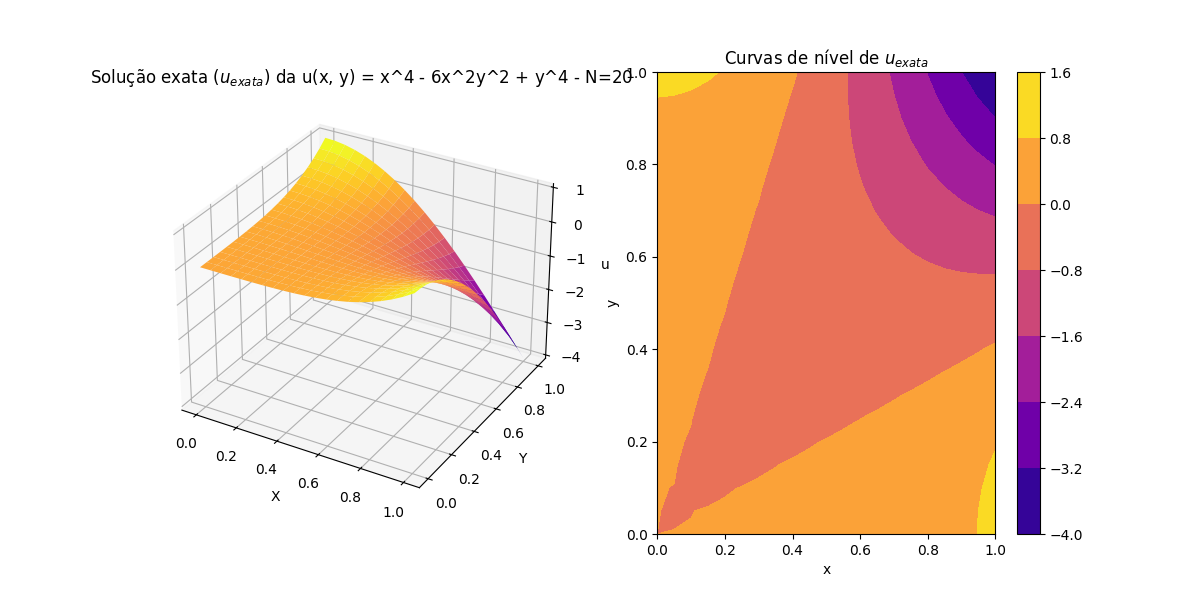
\includegraphics[width=\textwidth]{img/Problem1/a_20.png}
	      	      		\caption{Simulation 1A with $N = 20$}
	      	      	\end{minipage}
	      	      	\hfill
	      	      	\begin{minipage}{0.32\textwidth}
	      	      		\centering
	      	      		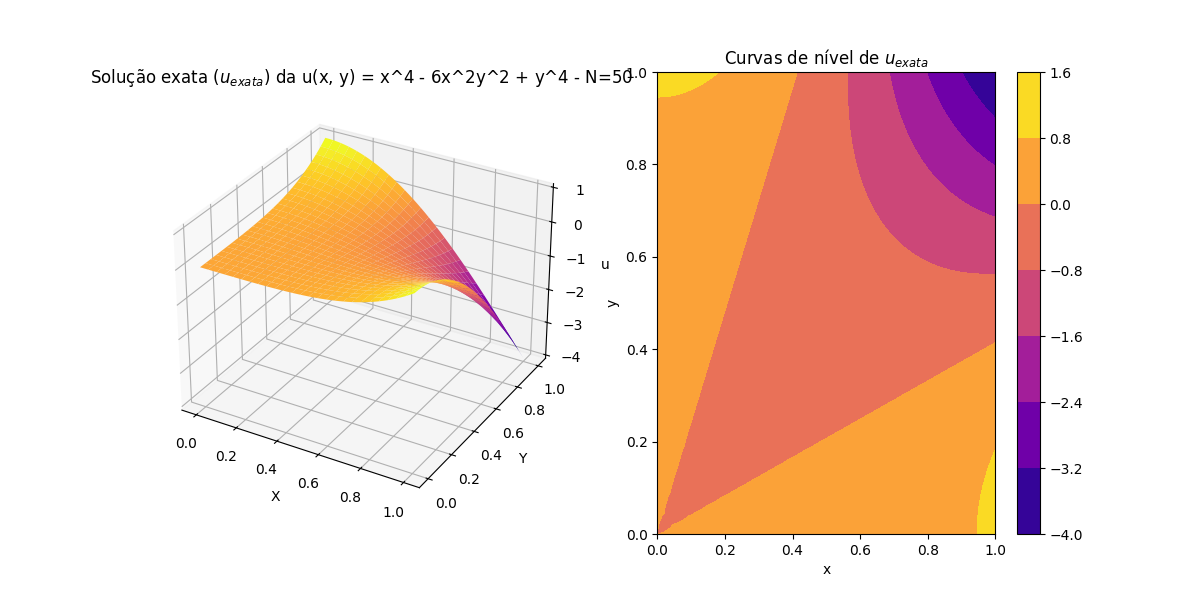
\includegraphics[width=\textwidth]{img/Problem1/a_50.png}
	      	      		\caption{Simulation 1A with $N = 50$}
	      	      	\end{minipage}
	      	      	\hfill
	      	      	\begin{minipage}{0.32\textwidth}
	      	      		\centering
	      	      		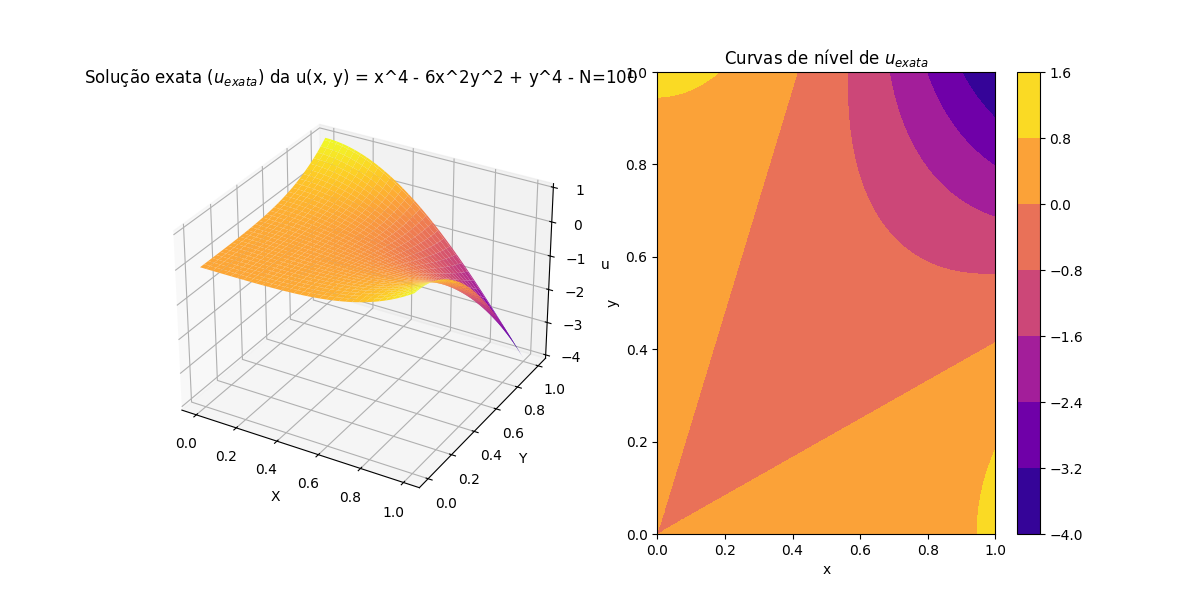
\includegraphics[width=\textwidth]{img/Problem1/a_100.png}
	      	      		\caption{Simulation 1A with $N = 100$}
	      	      	\end{minipage}
	      	      \end{figure}
	      	      
	      	\item $u(x,y) = e^x \sin(y)$
	      	      
	      	      \textbf{Solution:}
	      	      
	      	      \begin{figure}[H]
	      	      	\centering
	      	      	\begin{minipage}{0.32\textwidth}
	      	      		\centering
	      	      		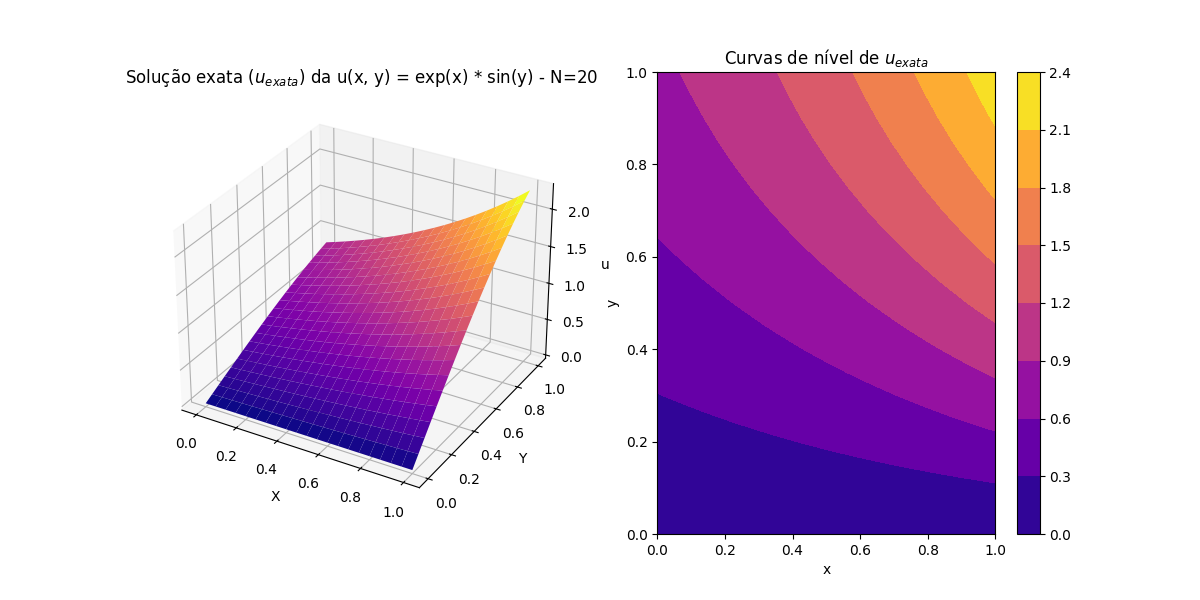
\includegraphics[width=\textwidth]{img/Problem1/b_20.png}
	      	      		\caption{Simulation 1B with $N = 20$}
	      	      	\end{minipage}
	      	      	\hfill
	      	      	\begin{minipage}{0.32\textwidth}
	      	      		\centering
	      	      		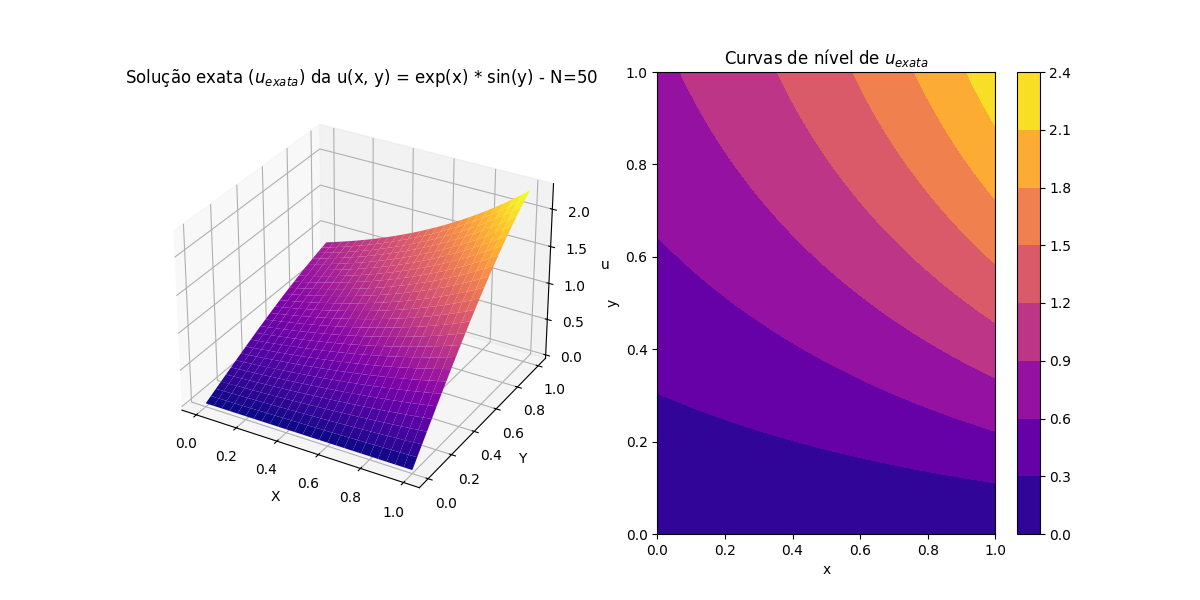
\includegraphics[width=\textwidth]{img/Problem1/b_50.png}
	      	      		\caption{Simulation 1B with $N = 50$}
	      	      	\end{minipage}
	      	      	\hfill
	      	      	\begin{minipage}{0.32\textwidth}
	      	      		\centering
	      	      		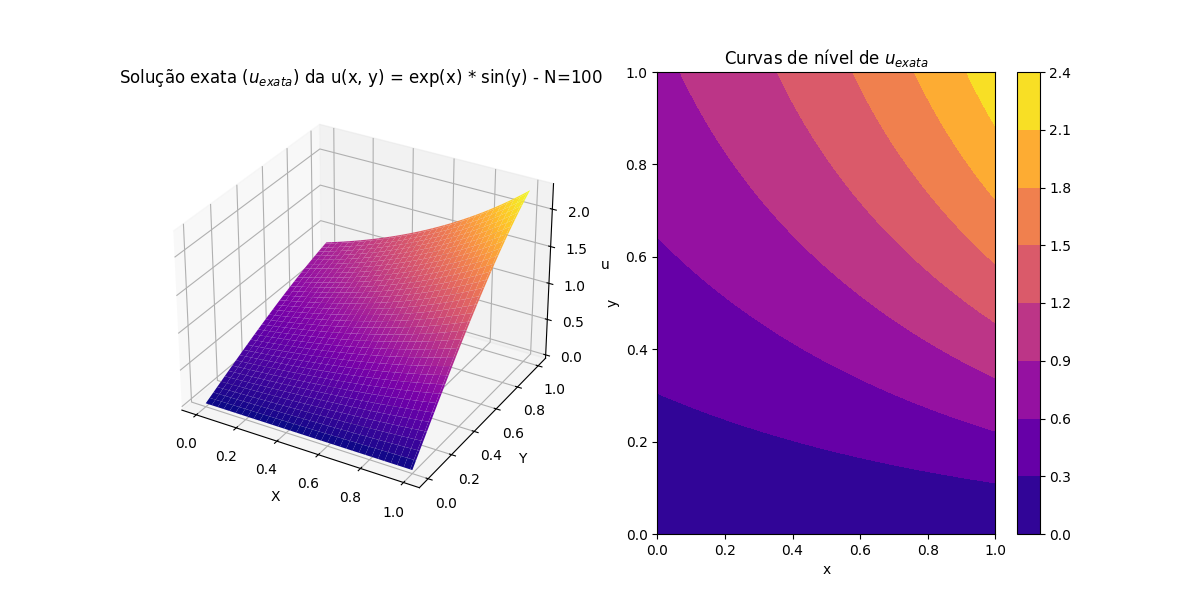
\includegraphics[width=\textwidth]{img/Problem1/b_100.png}
	      	      		\caption{Simulation 1B with $N = 100$}
	      	      	\end{minipage}
	      	      \end{figure}
	      \end{enumerate}
	      
	\item Consider the Poisson equation ($\Delta u = f$) on the unit square $\Omega = (0, 1) \times (0, 1)$ with the forcing function given by:
	      \begin{equation}
	      	f(x, y) = -2 \cos(x) \sin(y)
	      	\label{eq:enunciado-2a}
	      \end{equation}
	      
	      To solve this Poisson equation, we consider the exact solution:
	      \begin{equation}
	      	u_{\text{exact}}(x,y) = \cos(x)\sin(y)
	      	\label{eq:enunciado-2b}
	      \end{equation}
	      
	      Considering Dirichlet boundary conditions given by the exact solution:
	      \begin{enumerate}
	      	\item Verify that Equation \eqref{eq:enunciado-2b} satisfies the equation with the forcing function given in Equation \eqref{eq:enunciado-2a}
	      	      
	      	      To solve this question, we created a verification function as follows:
	      	      

	      	      \begin{lstlisting}
# Function to verify if the equation is satisfied
def verify() -> bool:
    # Define a grid of points for x and y in the interval [0, 1] with 5 divisions
    X = np.linspace(0, 1, 5)
    Y = np.linspace(0, 1, 5)
    
    # Loop through values of X and Y
    for x in X:  
        for y in Y:  
            left = f(x, y)  # left-hand side of the equation, value of f(x, y)
            right = -2 * np.cos(x) * np.sin(y)  # right-hand side of the equation

            # Check if the left side is approximately equal to the right side
            if not np.isclose(left, right):
                # If the values are not close, print an error with the corresponding x and y values
                print(f"Error: for (x={x}, y={y}), left = {left}, right = {right}")
                return False  # Return False to indicate that the equation is not satisfied
    
    return True  # The solution u(x, y) satisfies the equation with function f(x, y)
	      	      \end{lstlisting}
	      	      
	      	      Validating item (a) with this function, we get the following output:
	      	      
	      	      \begin{lstlisting}
print("Validating item (a)")
verify()
# -> True
	      	      \end{lstlisting}
	      	      
	      	\item Perform simulations for $N = 50, 100,$ and $200$, and plot both the numerical and exact solutions.
	      	      
	      	      \textbf{Solution:}
	      	      
	      	      \begin{figure}[H]
	      	      	\centering
	      	      	\begin{minipage}{0.32\textwidth}
	      	      		\centering
	      	      		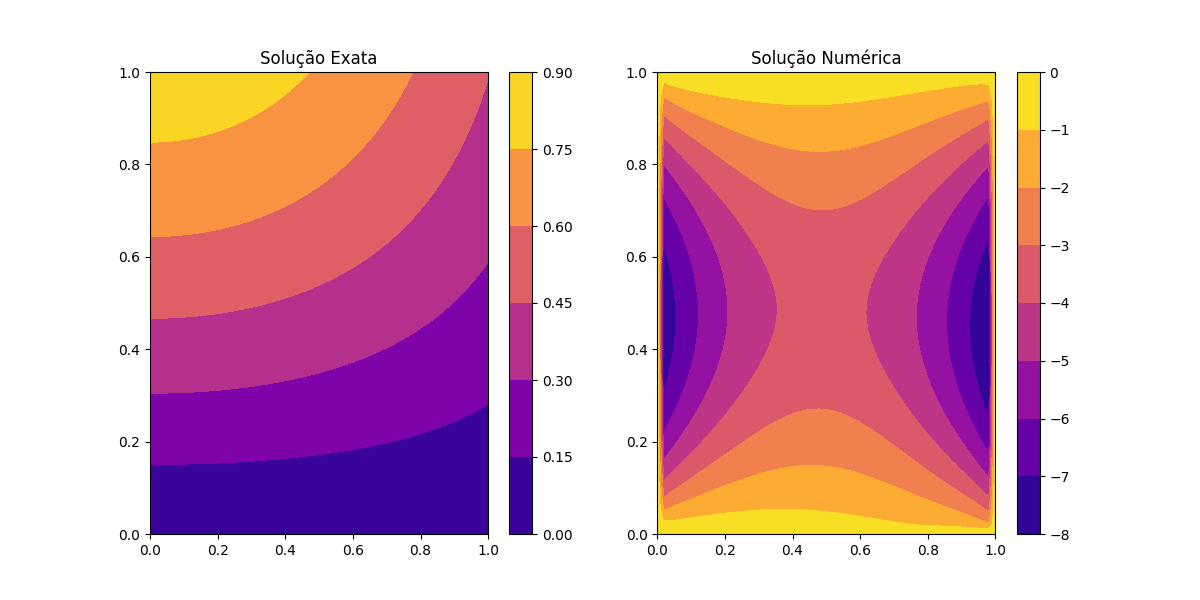
\includegraphics[width=\textwidth]{img/Problem2/50.png}
	      	      		\caption{Simulation 2B with $N = 50$}
	      	      	\end{minipage}
	      	      	\hfill
	      	      	\begin{minipage}{0.32\textwidth}
	      	      		\centering
	      	      		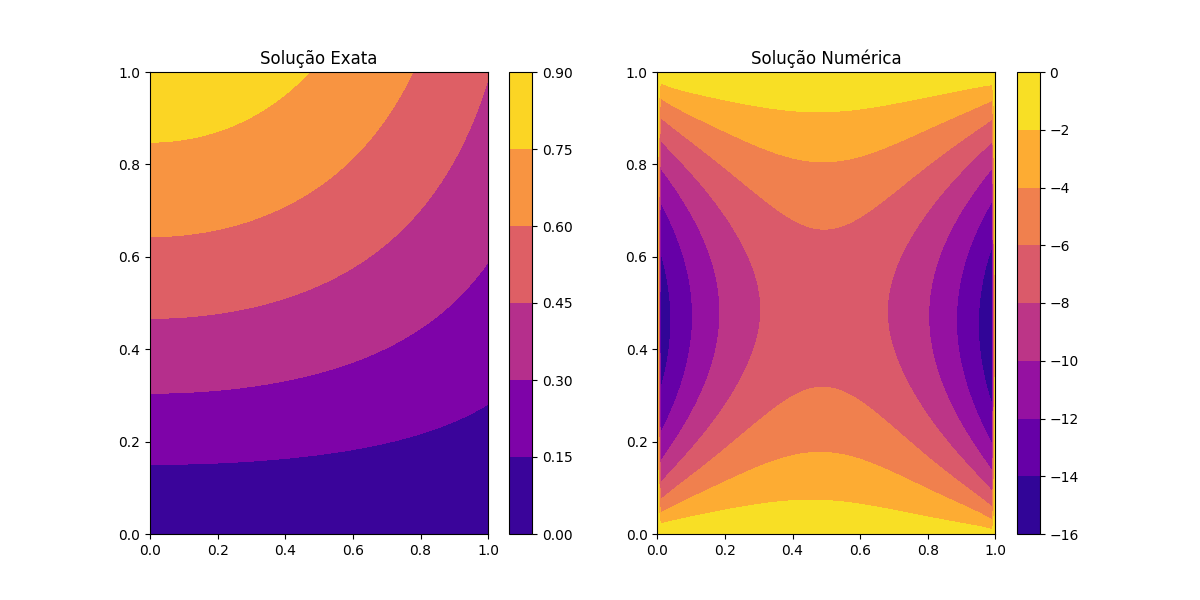
\includegraphics[width=\textwidth]{img/Problem2/100.png}
	      	      		\caption{Simulation 2B with $N = 100$}
	      	      	\end{minipage}
	      	      	\hfill
	      	      	\begin{minipage}{0.32\textwidth}
	      	      		\centering
	      	      		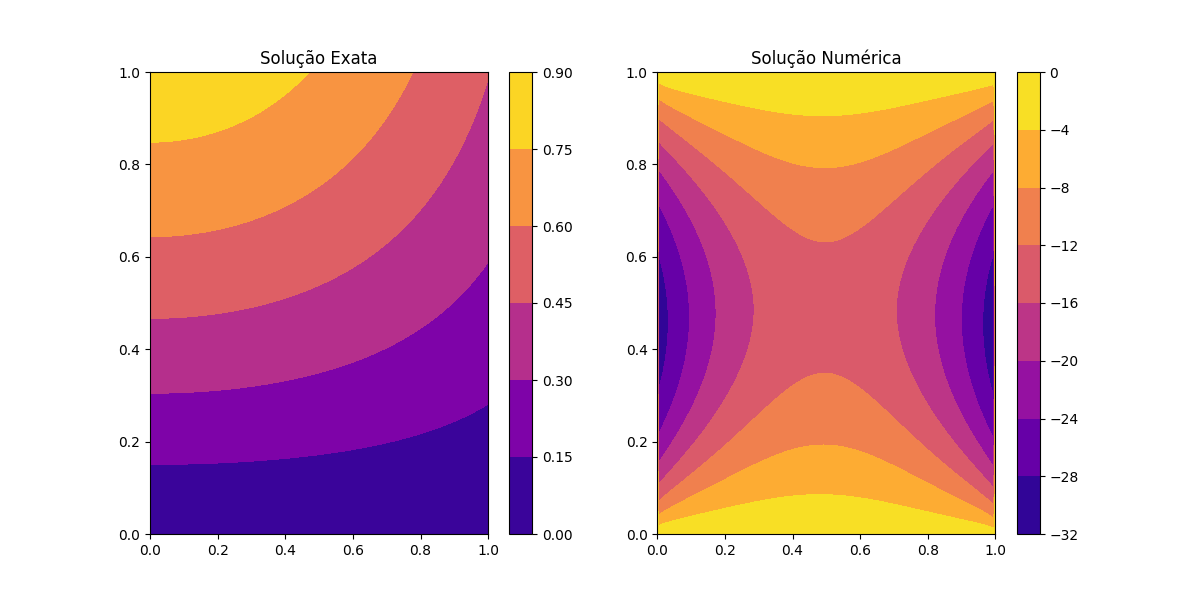
\includegraphics[width=\textwidth]{img/Problem2/200.png}
	      	      		\caption{Simulation 2B with $N = 200$}
	      	      	\end{minipage}
	      	      \end{figure}
	      	      
	      	\item Print the errors with respect to the continuous exact solution.
	      	      
	      	      \textit{Note: For this report, we present $20\%$ of the $x$ values and 4 values of $y$ for clarity. The full table is available in the accompanying code and attached \texttt{.csv} files.}
	      	      
	      	          
	      	      \begin{table}[H]
	      	      	\centering
	      	      	\caption{Error computed in the simulation for $N=50$}
	      	      	\label{tab:error_xy_50}
	      	      	\renewcommand{\arraystretch}{1.25}
	      	      	\setlength{\tabcolsep}{12pt}
	      	      	\begin{tabular}{|c|c|c|c|c|}
	      	      		\hline
	      	      		
	      	      		\textbf{$x$} & \textbf{$y = 0.00$} & \textbf{$y = 0.24$} & \textbf{$y = 0.47$} & \textbf{$y = 0.71$} \\ \hline
	      	      		0.00         & 0.000000            & 0.000000            & 0.000000            & 0.000000            \\ \hline
	      	      		0.10         & 0.099833            & 1.882937            & 1.616623            & 2.112684            \\ \hline
	      	      		0.20         & 0.198669            & 3.290300            & 2.644325            & 3.354436            \\ \hline
	      	      		0.29         & 0.295520            & 4.328647            & 3.445981            & 4.265023            \\ \hline
	      	      		0.39         & 0.389418            & 4.958013            & 3.957576            & 4.799946            \\ \hline
	      	      		0.49         & 0.479426            & 5.178478            & 4.148823            & 4.953132            \\ \hline
	      	      		0.59         & 0.564642            & 5.004041            & 4.017148            & 4.737323            \\ \hline
	      	      		0.69         & 0.644218            & 4.454460            & 3.582953            & 4.178380            \\ \hline
	      	      		0.78         & 0.717356            & 3.555614            & 2.888192            & 3.317695            \\ \hline
	      	      		0.88         & 0.783327            & 2.351951            & 1.997187            & 2.221227            \\ \hline
	      	      	\end{tabular}
	      	      \end{table}
	      	          
	      	      \begin{table}[H]
	      	      	\centering
	      	      	\caption{Error computed in the simulation for $N=100$}
	      	      	\label{tab:error_xy_100}
	      	      	\renewcommand{\arraystretch}{1.25}
	      	      	\setlength{\tabcolsep}{12pt}
	      	      	\begin{tabular}{|c|c|c|c|c|}
	      	      		\hline
	      	      		
	      	      		\textbf{$x$} & \textbf{$y = 0.00$} & \textbf{$y = 0.25$} & \textbf{$y = 0.50$} & \textbf{$y = 0.74$} \\ \hline
	      	      		0.00& 0.000000            & 0.000000            & 0.000000            & 0.000000\\ \hline
	      	      		0.05         & 0.049979            & 1.800425            & 1.580714            & 2.211568            \\ \hline
	      	      		0.10         & 0.099833            & 3.290075            & 2.649791            & 3.674547            \\ \hline
	      	      		0.15         & 0.149438            & 4.663765            & 3.657335            & 5.017072            \\ \hline
	      	      		0.20         & 0.198669            & 5.883958            & 4.577122            & 6.202277            \\ \hline
	      	      		0.25         & 0.247404            & 6.927325            & 5.386953            & 7.208167            \\ \hline
	      	      		0.30         & 0.295520            & 7.781173            & 6.069078            & 8.023337            \\ \hline
	      	      		0.35         & 0.342898            & 8.439803            & 6.610197            & 8.643080            \\ \hline
	      	      		0.40         & 0.389418            & 8.901834            & 7.001193            & 9.066735            \\ \hline
	      	      		0.45         & 0.434966            & 9.168515            & 7.236726            & 9.296104            \\ \hline
	      	      		0.50         & 0.479426            & 9.242750            & 7.314824            & 9.334585            \\ \hline
	      	      		0.54         & 0.522687            & 9.128568            & 7.236536            & 9.186741            \\ \hline
	      	      		0.59         & 0.564642            & 8.830868            & 7.005679            & 8.858139            \\ \hline
	      	      		0.64         & 0.605186            & 8.355364            & 6.628709            & 8.355390            \\ \hline
	      	      		0.69         & 0.644218            & 7.708736            & 6.114688            & 7.686390            \\ \hline
	      	      		0.74         & 0.681639            & 6.899043            & 5.475334            & 6.860820            \\ \hline
	      	      		0.79         & 0.717356            & 5.936584            & 4.725096            & 5.891004            \\ \hline
	      	      		0.84         & 0.751280            & 4.835443            & 3.881186            & 4.793198            \\ \hline
	      	      		0.89         & 0.783327            & 3.615889            & 2.963487            & 3.589201            \\ \hline
	      	      		0.94         & 0.813416            & 2.307188            & 1.994244            & 2.307665            \\ \hline
	      	      	\end{tabular}
	      	      \end{table}
	      	          
	      	          
	      	      \begin{table}[H]
	      	      	\centering
	      	      	\caption{Error computed in the simulation for $N=200$}
	      	      	\label{tab:error_xy_200}
	      	      	\renewcommand{\arraystretch}{1.25}
	      	      	\setlength{\tabcolsep}{12pt}
	      	      	\begin{tabular}{|c|c|c|c|c|}
	      	      		\hline
	      	      		
	      	      		\textbf{$x$} & \textbf{$y = 0.00$} & \textbf{$y = 0.25$} & \textbf{$y = 0.50$} & \textbf{$y = 0.75$} \\ \hline
	      	      		0.00         & 0.000000            & 0.000000            & 0.000000            & 0.000000            \\ \hline
	      	      		0.02         & 0.019999            & 1.461875            & 1.337067            & 1.886796            \\ \hline
	      	      		0.04         & 0.039989            & 2.667926            & 2.190556            & 3.083192            \\ \hline
	      	      		0.06         & 0.059964            & 3.857494            & 3.035968            & 4.262617            \\ \hline
	      	      		0.08         & 0.079915            & 5.023001            & 3.869449            & 5.417385            \\ \hline
	      	      		0.10         & 0.099833            & 6.157533            & 4.687248            & 6.540515            \\ \hline
	      	      		0.12         & 0.119712            & 7.254949            & 5.485749            & 7.625847            \\ \hline
	      	      		0.14         & 0.139543            & 8.309931            & 6.261493            & 8.668087            \\ \hline
	      	      		0.16         & 0.159318            & 9.317985            & 7.011203            & 9.662789            \\ \hline
	      	      		0.18         & 0.179030            & 10.275386           & 7.731804            & 10.606301           \\ \hline
	      	      		0.20         & 0.198669            & 11.179117           & 8.420429            & 11.495686           \\ \hline
	      	      		0.22         & 0.218230            & 12.026776           & 9.074439            & 12.328629           \\ \hline
	      	      		0.24         & 0.237703            & 12.816498           & 9.691418            & 13.103346           \\ \hline
	      	      		0.26         & 0.257081            & 13.546865           & 10.269181           & 13.818498           \\ \hline
	      	      		0.28         & 0.276356            & 14.216838           & 10.805773           & 14.473115           \\ \hline
	      	      		0.30         & 0.295520            & 14.825685           & 11.299460           & 15.066528           \\ \hline
	      	      		0.32         & 0.314567            & 15.372932           & 11.748732           & 15.598318           \\ \hline
	      	      		0.34         & 0.333487            & 15.858310           & 12.152287           & 16.068264           \\ \hline
	      	      		0.36         & 0.352274            & 16.281724           & 12.509030           & 16.476315           \\ \hline
	      	      		0.38         & 0.370920            & 16.643219           & 12.818060           & 16.822552           \\ \hline
	      	      		0.40         & 0.389418            & 16.942954           & 13.078665           & 17.107171           \\ \hline
	      	      		0.42         & 0.407760            & 17.181186           & 13.290309           & 17.330460           \\ \hline
	      	      		0.44         & 0.425939            & 17.358254           & 13.452628           & 17.492789           \\ \hline
	      	      		0.46         & 0.443948            & 17.474564           & 13.565421           & 17.594595           \\ \hline
	      	      		0.48         & 0.461779            & 17.530584           & 13.628641           & 17.636378           \\ \hline
	      	      		0.50         & 0.479426            & 17.526836           & 13.642390           & 17.618691           \\ \hline
	      	      		0.52         & 0.496880            & 17.463888           & 13.606916           & 17.542140           \\ \hline
	      	      		0.54         & 0.514136            & 17.342356           & 13.522605           & 17.407378           \\ \hline
	      	      		0.56         & 0.531186            & 17.162898           & 13.389980           & 17.215108           \\ \hline
	      	      		0.58         & 0.548024            & 16.926217           & 13.209698           & 16.966079           \\ \hline
	      	      		0.60         & 0.564642            & 16.633058           & 12.982549           & 16.661093           \\ \hline
	      	      		0.62         & 0.581035            & 16.284216           & 12.709451           & 16.301004           \\ \hline
	      	      		0.64         & 0.597195            & 15.880535           & 12.391458           & 15.886728           \\ \hline
	      	      		0.66         & 0.613117            & 15.422918           & 12.029754           & 15.419245           \\ \hline
	      	      		0.68         & 0.628793            & 14.912336           & 11.625655           & 14.899616           \\ \hline
	      	      		0.70         & 0.644218            & 14.349838           & 11.180616           & 14.328987           \\ \hline
	      	      		0.72         & 0.659385            & 13.736566           & 10.696224           & 13.708612           \\ \hline
	      	      		0.74         & 0.674288            & 13.073777           & 10.174208           & 13.039867           \\ \hline
	      	      		0.76         & 0.688921            & 12.362868           & 9.616434            & 12.324278           \\ \hline
	      	      		0.78         & 0.703279            & 11.605403           & 9.024911            & 11.563548           \\ \hline
	      	      		0.80         & 0.717356            & 10.803155           & 8.401786            & 10.759585           \\ \hline
	      	      		0.82         & 0.731146            & 9.958146            & 7.749346            & 9.914547            \\ \hline
	      	      		0.84         & 0.744643            & 9.072699            & 7.070015            & 9.030875            \\ \hline
	      	      		0.86         & 0.757843            & 8.149492            & 6.366347            & 8.111341            \\ \hline
	      	      		0.88         & 0.770739            & 7.191612            & 5.641024            & 7.159079            \\ \hline
	      	      		0.90         & 0.783327            & 6.202604            & 4.896841            & 6.177620            \\ \hline
	      	      		0.92         & 0.795602            & 5.186507            & 4.136700            & 5.170910            \\ \hline
	      	      		0.94         & 0.807558            & 4.147869            & 3.363597            & 4.143303            \\ \hline
	      	      		0.96         & 0.819192            & 3.091718            & 2.580601            & 3.099536            \\ \hline
	      	      		0.98         & 0.830497            & 2.023504            & 1.790843            & 2.044666            \\ \hline
	      	      	\end{tabular}
	      	      \end{table}
	      \end{enumerate}
\end{enumerate}

\section{Conclusion}

In this work, we explored the numerical solution of the Poisson equation using the finite difference method in a unit domain, under Dirichlet boundary conditions. The implementation successfully produced numerical solutions for different values of $N$, and we observed the convergence of the error as the mesh spacing decreased.

The analysis of the error tables showed that, for larger values of $N$, the absolute error computed at points in the domain decreased significantly, confirming the method’s efficiency. For instance, when $N = 20$, the error was more noticeable, especially near the domain boundaries. However, increasing $N$ to $50$ and $100$ considerably reduced the error, demonstrating the consistency of the method and the convergence of the numerical solution toward the exact one as the mesh became finer.

Throughout the process, we identified important aspects related to error estimation and method consistency. One key point was the importance of properly defining the boundary conditions, which have a direct impact on the results obtained.

In summary, this study provided a deeper understanding of the application of numerical methods to differential equations, demonstrating the effectiveness of the finite difference method and the importance of error analysis in validating numerical solutions.

\renewcommand{\bibsection}{}

\section{References}
\nocite{*}
\bibliographystyle{abbrv}
\bibliography{referencias}

\end{document}
